\documentclass[10pt,twocolumn,letterpaper]{article}

\usepackage{iccv}
\usepackage{times}
\usepackage{epsfig}
\usepackage{graphicx}
\usepackage{amsmath}
\usepackage{amssymb}

% Include other packages here, before hyperref.

% If you comment hyperref and then uncomment it, you should delete
% egpaper.aux before re-running latex.  (Or just hit 'q' on the first latex
% run, let it finish, and you should be clear).
\usepackage[breaklinks=true,bookmarks=false]{hyperref}

\iccvfinalcopy % *** Uncomment this line for the final submission

\def\iccvPaperID{****} % *** Enter the ICCV Paper ID here
\def\httilde{\mbox{\tt\raisebox{-.5ex}{\symbol{126}}}}

% Pages are numbered in submission mode, and unnumbered in camera-ready
%\ificcvfinal\pagestyle{empty}\fi
\setcounter{page}{1}
\begin{document}

%%%%%%%%% TITLE
\title{Add Named Entity Recognizer to Convolutional Neural Network }

\author{
Guangyu Lin\\
UTEID: gl8429\\
{\tt\small glin@utexas.edu} \\
\and
Ge Gao\\
UTEID: gg24984\\
{\tt\small gegao1118@utexas.edu} \\
\and
Huihuang Zheng\\
UTEID: hz4674\\
{\tt\small huihuang@utexas.edu} \\
}
% For a paper whose authors are all at the same institution,
% omit the following lines up until the closing ``}''.
% Additional authors and addresses can be added with ``\and'',
% just like the second author.
% To save space, use either the email address or home page, not both
%\and
%Second Author\\
%Institution2\\
%First line of institution2 address\\
%\tt\small secondauthor@i2.org}
%}

\maketitle
%\thispagestyle{empty}


%%%%%%%%% ABSTRACT
\begin{abstract}
In this work, our assumption is that adding Named Entity Recognizor (NER) \cite{nadeau2007survey} as a feature for Convoluional Neural Network can improve accuracy for NLP tasks involving named entities. To verify our assumption, we try to solve TREC question classification task \cite{li2002learning}. Our method adds Named Entity Recognizor (NER) as one dimension number to \textit{word2vec} expression, then the modified expression is used for training a CNN. Our experiment illustrated that our CNN + NER model can improve the accuracy of question type classification task compared to only CNN method. Although our method still can not get comparable performance of the state-of-the-art work, Our method is easier to train because the state-of-the-art work needs a large number of hand-code resources. 
\end{abstract}

%%%%%%%%% BODY TEXT

\section{Introduction}
Automatic question answering is an important information retrieval task in natural language processing and it is more challenging than purely searching task because it needs to ``understand'' what is asked before searching for answers. And to make machines ``understand'' a question is as challenging as it sounds like. One method that could help solve this problem is called Question Classification(QC). Question Classification(QC) is a task that given a question, some classifier will map this question to one of k limited classes, so that some semantic constraint will be put on this question, which provides machine with some basic information about the question which could hopefully help machine ``understand'' questions.

In 2000's TREC competition \cite{li2002learning}, participants were requested to develop a system to classify English questions based on some question categories. And after that, many remarkable results have been achieved. One of them is Li and Roth's work. Li and Roth develops a hierarchical classifier based on SNoW learning architecture(Carlson et al, 1999 \cite{carlson1999snow}; Roth, 1998 \cite{roth1998learning}) to solve the question classification task.

With the development of deep learning, machine learning models have been applied to NLP tasks and it turns out that many of these models significantly improved performance of original models without deep learning methods. One example is Yoon Kim's \cite{kim2014convolutional} work that applies convolutional neural networks (CNN) to sentence classification.

Since named entity is an important part of questions, especially when number of question types is large, but previous work did not make much use of the semantic information of a named entity. For example the named entity might be either a location or a person. This work makes use of Stanford's Named Entity Recognizer (NER) \cite{nadeau2007survey} and adds extra labels to vectors generated by \textit{word2vec}. Then we train convolutional neural network model with these new vectors. Our goal is to improve the performance of the CNN model for question classification, especially for questions related to named entity semantic meanings.

The main contribution of this work is that our method, which adds Name Entity Recognizer (NER) as one extra dimension for each \textit{word2vec}'s output vector, can improve top-1 accuracy in a 50-classes question classification task -- TREC fine types, which demonstrates that by combining NER and CNN, our method can improve CNN classification accuracy. Although our method still cannot outperform the state-of-the-art method which doesn't apply neural networks, our CNN classifier is easier to deploy because the non-neural approach method uses a large number of hand-coded resources. 

\section{Problem Definition and Algorithm}
\subsection{Task Definition}
Many problems of natural language processing can be viewed as problems of resolving ambiguity, which is based on properties of the surrounding context, which are syntactic or semantic. For example, the problem of Question Answering(QA). QA problem is different from querying answers from search engine because we need to give a accurate and concise answer to a free-form factual question. Therefore, advanced natural language techniques rather than key term extraction and expansion are needed. We can also treat this problem as a natural language understanding problem. We can solve Question Answering problem by solving Question Classification (QC) problem. We define QC to be a multi-classification task that seeks a mapping g : Q $\rightarrow$ \{${c_1}$,..., ${c_n}$\} from an instance q $\in$ Q to one of n classes ${c_1}$,..., ${c_n}$. In order to improve the accuracy of QC, we would like an algorithm combination with Named Entity Recognition, Word2Vec and Convolutional Neural Network.

\subsection{Algorithm}
\subsubsection{Named Entity Recognition}
Named Entity Recognition (NER) \cite{finkel2005incorporating}labels sequences of words in a text which are the names of things, such as person and company names, or gene and protein names. All named entities are self-explanatory in Tabel ~\ref{tab:1}. As named entity recognition is frequently a prelude to identifying relations in Information Extraction, it can also contribute to other tasks. For example in our Question Answering(QA), we can improve the accuracy of our question classifiers by recovering not whole pages, but just those parts which contain an answer to the user's question. For example, we have a question, \\\\{\bf "How did serfdom develop in and then leave Russia ?"} \\\\Although this is a particular question about a description of manner, this is also a question to query something related to Russia, which is a named entity - LOCATION. While searching the correct answer, it will help us skip very wrong answer if we can combine with the location named entity. Therefore we would like to use Named Entity Recogniser to preprocess our data in order to help our classifier skip very wrong answer.
	\begin{table}[!hbt]
	\resizebox{\linewidth}{!}{
		\begin{tabular}{|c|c|}
			\hline
			NE Type & Examples \\ \hline
			  ORGANIZATION  & Georgia-Pacific Corp., WHO \\ \hline
			  PERSON  & Eddy Bonte, President Obama \\ \hline
			  LOCATION  & Murray River, Mount Everest \\ \hline
			  DATE  & June, 2008-06-29 \\ \hline
			  TIME  & two fifty a m, 1:30 p.m. \\ \hline
			  MONEY  & 175 million Canadian Dollars, GBP 10.40 \\ \hline
			  PERCENT  & twenty pct, 18.75 \%\\ \hline
			 \hline
		\end{tabular}
		}
		\caption{NER}
		\label{tab:1}
	\end{table}

In Figure.~\ref{fig:pipeline}, we present a simple pipeline architecture for an named entity recognition system. However, we would like to use Stanford Named Entity Recognizer (NER) to retrieve named entity from our sentences. Because they train a large corpus and have a good performance.
\begin{figure}
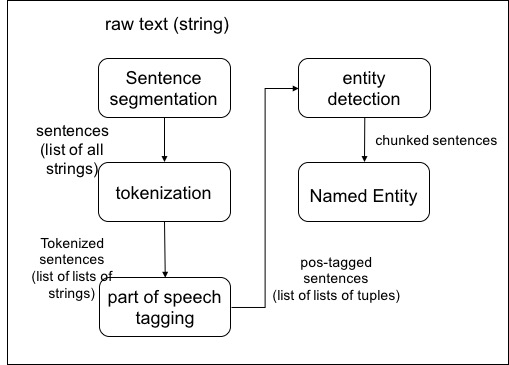
\includegraphics[width=\linewidth]{pipeline}
\caption{Simple Pipeline Architecture for an Named Entity Recognition System. }
\label{fig:pipeline}
\end{figure}

\subsubsection{Word2Vec}
Word2vec is a two-layer neural net that processes text. Its input is a text corpus and its output is a set of vectors: feature vectors for words in that corpus. We use word2vec to turn text into a numerical form that convonlutional neural network can understand. The output of the word2vec is a vocabulary in which each item has a vector attached to it. We can also easily store this model and reload this model in the later. In order to visualise the result of word2vec, we present an example on the website. Here?s a list of words associated with "Sweden" using Word2vec, in order of proximity. Here is in Figure.~\ref{fig:word2vec}.

\begin{figure}
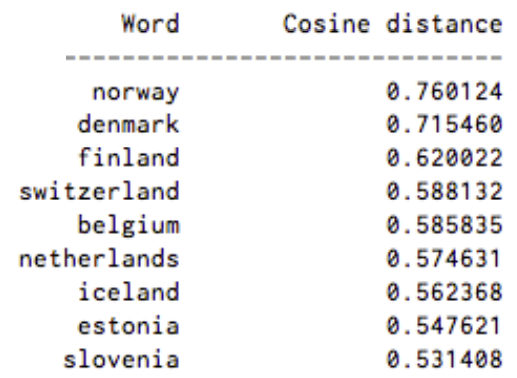
\includegraphics[width=\linewidth]{word2vec}
\caption{Simple Pipeline Architecture for an Named Entity Recognition System. }
\label{fig:word2vec}
\end{figure}
The nations of Scandinavia and several wealthy, northern European, Germanic countries are among the top nine. \cite{bahrampour2015comparative}
In our experiment, we would like to use word2vec to train our sentence and get each word as a vector v, then prepare it for convolutional neural network.

\subsubsection{Convolutional neural network}
After we get vector $v$ for each word where the $v \in \mathbb{R}^k$ is the $k$-dimensional word vector, we use Kim's CNN architecture. A sentence of length $n$ (padded where necessary) is represented as concatenation of word vectors:
$$v_{1:n} = v_1 \oplus v_2 \oplus v_3 ... \oplus v_n$$
where $v_i$ is corresponding to the $i$-th word in the sentence. 

In general, let $v_{i:i+j}$ refers to the concatenation of word vectors $v_i, v_{i+1}, ..., v_{i+j}$. We will describe how one filter extracts feature and then discuss the CNN with multiple convolutional filters. A convolutional filter of Convolutional Neural Network (CNN)  \cite{kim2014convolutional} takes fixed size of input of $\mathbb{R}^{hk}$. A convolutional filter $w \in \mathbb{R}^{hk}$ is applied to each possible window of words of the sentence $\{x_{1:h}, x_{2:h+1}, ..., x_{n-h+1:n}\}$. The features are extracted as
$$c_i = f(w  x_{i:i+h-1} + b)$$
So convolutional layer produce a feature map:
$$c = [c_1, c_2, ... c_{n-h+1}]$$
 
Then, we applied a max pooling over the feature map and take the maximum value:
$$\hat{c} = \max \{c\}$$
The idea is to capture the most important feature.

Above we describe the process how one feature was extracted by convolutional neural network by one filter. In fact, the model has multiple filters so it extracts multiple features. These features from the penultimate layer and are passed to a fully connected softmax layer whose output is the probability distribution over labels. Figure \ref{cnn} shows an

\begin{figure*}
  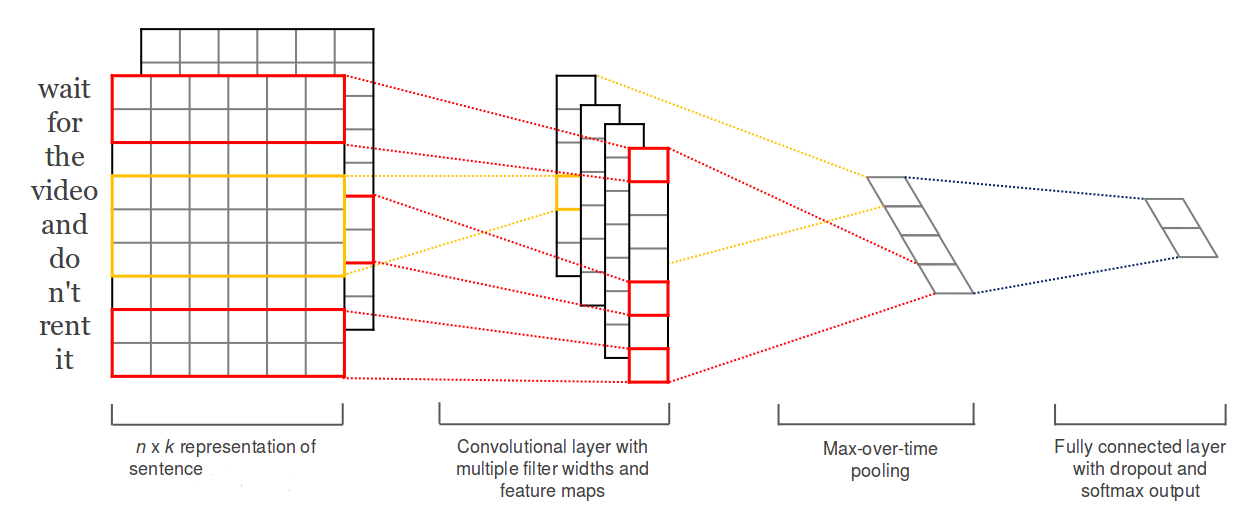
\includegraphics[width=\linewidth]{cnn.png}
  \caption{CNN model example}
  \label{cnn}
\end{figure*}


\subsubsection{Our Approach}
We add \textit{Name Entity Recognizor} (NER) to the word expression $v$. Let our word vector be $v' \in \mathbb{R}^{k+1}$. We are going to add one dimension to \textit{word2vec} expression. Let
$$v' = [v, e]$$
where $v$ is the output vector of \textit{word2vec} and $e$ is the label number indicating the named entity. Then we will modify CNN architectures: add one input dimension and keep others the same as previous CNN. Suppose previous CNN convolutional filters take input of $\mathbb{R}^{kh}$ and we will change input size into $\mathbb{R}^{(k+1)h}$. 

Figure \ref{process} shows an figure illustration of our approach.
 
\begin{figure}
  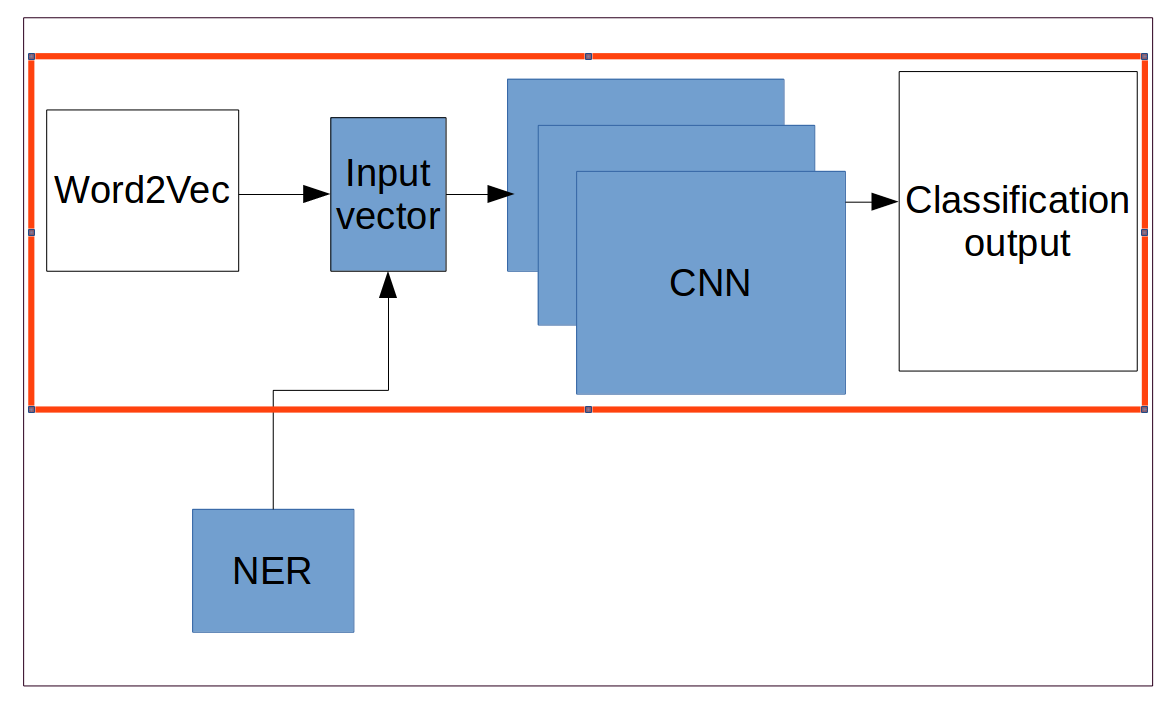
\includegraphics[width=\linewidth]{process.png}
  \caption{Our Approach: Red Rectangle marked the traditional method and Blue Boxes are where we changed}
  \label{process}
\end{figure}




\section{Experiment}
\subsection{Methodology}

\subsubsection{Dataset}
Our method was evaluated by comparing accuracy in a question classification task named TREC \cite{li2006learning} with previous researchers' results. The task involves classifying a question into $k$ question types. They defined a two-layered taxonomy, which represents a  natural semantic classification for typical answers in the TREC task. The hierarchy contains 6 coarse classes (ABBREVIATION, ENTITY, DESCRIPTION, HUMAN, LOCATION and NUMERIC VALUE) and 50 fine classes. Each coarse  class contains a non-overlapping set of fine classes. We choose this dataset because of two reasons. The fact that Named Entity Recognizer can classify person, location may help us in this task. Second, in Kim's paper \cite{kim2014convolutional} and Li's paper \cite{li2006learning}, they also used this database and reported previous accuracy so it will be easy for us to compare. The TREC dataset has 5500 annotated questions for training and 500 questions as the test set.

\subsubsection{Setup}
We used \textit{word2vec} trained model from Mikolov \cite{mikolov2013efficient} on 100 billion words of Google News and from \cite{mikolov2014word2vec}. We built our framework using NER from Stanford NER software \cite{finkel2005incorporating}

and deep learning tool Theano \cite{Bastien-Theano-2012}. Since Kim's work\cite{kim2014convolutional} has Github published code using Theano (\url{https://github.com/yoonkim/CNN_sentence}), our method which combines CNN and NER was extended from their code. 

We compared our method with Kim's method of using CNN and previous best methods without using CNN in the TREC dataset. By comparing CNN and our CNN + NER method, we can evaluate the contribution of NER features in this task. In addition, because Kim's method didn't outperform previous methods without CNN, we need to compare previous methods.

\subsubsection{Evaluation}
In this paper, we use same metric as previous researchers. We count the number of correctly classified questions by two standards. Top-1 accuracy and top-5 accuracy. We define
$$ 
I_{i,j} = 
\left\{ 
  \begin{array}{ll}
    1 & \parbox{5cm}{Correct label of the $i$-th question is output within rank $j$ }\\
    \\
    0 & \parbox{3cm}{otherwise}
  \end{array} 
\right. 
$$
Here, classifiers will give $j$ labels for the $i$-th question. If the correct label for question $i$ is among those $j$ labels, $I_{i,j}$ will be set to 1. Top 1 accuracy is defined as $j = 1$, which is a usual precision definition. Top 5 accuracy is defined as $j = 5$, which allows multi-labels for classifiers. Formally, if we have n test samples, top-$k $ accuracy is defined as
$$
P_k = \frac{1}{n}\sum_{i=1}^{n} I_{i,k} 
$$

\subsection{Experimental Results}
We reimplemented Kim's CNN method as baseline. We train Kim's CNN and our CNN + NER in 2000 epochs. Then, we record the best accuracy in the 2000 epochs. Our result uses non-static CNN in Kim's paper because it got best result than other Kim's CNN model in this task. We compared with two methods without using CNN: 1, Hierarchical classifier by Li and Roth\cite{li2002learning} uses features unigram, POS, head chunks, NE, and semantic relations. 2, SVM$_s$ uses ni-bi-trigrams, wh word, head word, POS, parser, hypernyms, and 60 hand-coded rules as features from Silva et al \cite{silva2011symbolic}, which is the state-of-the-art in the best of our knowledge. Our test result for coarse classes was shown in table \ref{coarse}. Our test result for fine classes was shown in table \ref{fine}

\begin{table}
\resizebox{\linewidth}{!}{
\begin{tabular}{|c|c|c|}
  \hline  
  Method & Top-1 Accuracy & Top-5 Accuracy\\
  \hline
  Hierarchical classifier\cite{li2002learning} & 91.0 & 98.8 \\
  SVM$_S$ \cite{silva2011symbolic} & 95.0 & - \\
  %DCNN \cite{kalchbrenner2014convolutional} & 93.0 & - \\
  CNN \cite{kim2014convolutional} & 91.8 & 100.0 \\
  \hline
  CNN + NER (ours) & 91.8 & 100.0 \\
  \hline
\end{tabular}
}
\caption{Top-1 and top-5 accuracy for TREC coarse question types. }
\label{coarse}
\end{table}

\begin{table}

\resizebox{\linewidth}{!}{
\begin{tabular}{|c|c|c|}
  \hline  
  
  Method & Top-1 accuracy & Top-5 accuracy\\
  \hline
  Hierarchical classifier\cite{li2002learning} & 84.20 & 95.00 \\
  SVM$_S$ \cite{silva2011symbolic} & 90.8 & - \\
  CNN \cite{kim2014convolutional} & 80.2 & 90.60 \\
  \hline
  CNN + NER (ours) & 81.0 &  90.60 \\ 
  \hline
\end{tabular}
}
\caption{Top-1 and top-5 accuracy for TREC coarse question types.}
\label{fine}
\end{table}

\subsection{Discussion}
In table \ref{coarse}, we can see our CNN + NER model doesn't improve accuracy from Kim's only CNN model. However, when it is in a more complexed situation, the fine task in table \ref{fine}, we can see our model can slightly improved the top-1 accuracy (81.0 vs 80.2 in only CNN model). 

Comparing to non-neural approaches methods, which needs manually engineered features. CNN's approach is easier to train. Our method has higher top-1 and top-5 accuracy than the Hierarchical classifier method in coarse task. However in fine task, Li and Roth's method outperforms ours. According to the fact that we add NER's feature to CNN and improved the accuracy of fine task, we think that demonstrates the human defined features are helpful in fine types classification. 

Our CNN + NER model has not got comparable accuracy to the work of Silva et al. \cite{silva2011symbolic}. However, their classifier involves a large number of hand-code resources. For example, they have 60 hand-coded rules. CNN's training is simpler because we don't need those manually engineered features. 

\section{Related Work}
\subsection{Question classifiers}
In the ``Learning Question Classifier'' paper (Li and Roth, 2002 \cite{li2002learning}), in terms of the question classification task, the number of question types(k) could be either six or fifty depending on different classification criteria.  Li and Roth developed a machine learning method to classify questions, which is guided by a layered semantic hierarchy of answer types. They made use of a sequence of two simple classifiers to do the classification. The first classifies questions into coarse classes (six in total) and the second classifies questions into fine classes (fifty in total), which is dependent on the first one. Here is the structure of the hierarchical classifier by Li and Roth.
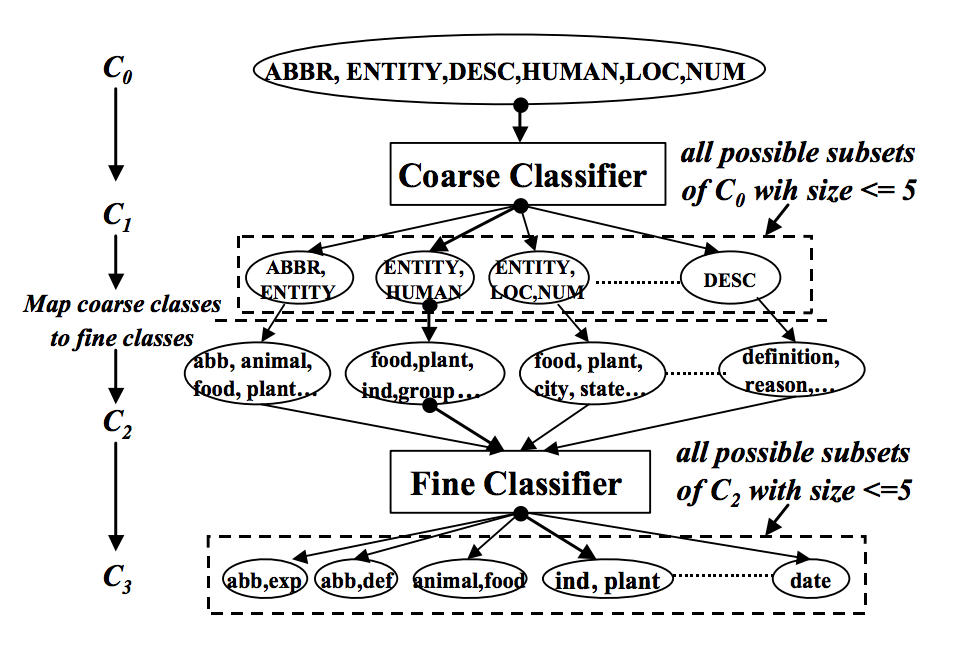
\includegraphics[width=0.5\textwidth]{structure.png}
\begin{center}
Figure1:  The hierarchical classifier 
\end{center}
Figure 1 shows the basic classification process by classifier developed by Li and Roth. A question will always be processed along a top-down path to be classified. And after the classification process, question type label(s) will be attached to the question.

In Li and Roth's classifier, each question is analyzed as a list of features so that they could be trained and tested for learning. They extracted some primitive features like words, pos tags and chunks (Abney, 1991 \cite{berwick1991principle}), named entity as well as some semantically related words. Based on these features, they compose and make some more complex features. Also, they make a semantically related word list for each of most question types. For example, ``far'' is in the semantically related words of ``distance'' so that if there is an occurrence of ``far'', and then the sensor for ``distance'' will be activated and the feature will be extracted.

A point that is worth pointing out is that there might be ambiguity for some specific questions. For example, a question like ``What do bats eat'' could either be classified to belong to food type or animal type, and both them make much sense. To solve this, Li and Roth allow multiple type labels to be attached to a single question.

\subsection{CNN on sentences classification}
Convolutional neural networks (CNN) model is a deep learning method which has achieved remarkable results in many fields. A CNN model was developed by Yoon Kim \cite{kim2014convolutional} for sentence classification which accepts word vectors as input and generates type labels as output.

Convolutional neural networks was originally invented for tasks in computer vision fields and was proved to be also effective in many NLP tasks. In Kim' model, they train one layer of filter on top of word vectors generated by word2vec developed by Google (Mikolov et al 2013 \cite{mikolov2013efficient}). In Kim's model, there are ``static'' and ``nonstatic'' models for model variation, where ``static'' means that the vectors are directly from word2vec and for ``nonstatic'', those vectors will also be tuned for each data set.


\section{Future Work}
This time we tried add NER features to CNN and improved CNN question classifier slightly, we think if we add more features, the CNN classifier can be more accurate.

\section{Conclusion}
In this work, we add Named Entity Recognizor (NER) as one dimension number to \textit{word2vec} expression. The modified expression can be used for training a CNN for NLP tasks involving named entity. Our experiment shows that our CNN + NER model can improve the accuracy of question type classification task compared to only CNN method. Although our method still can not get comparable performance of the state-of-the-art work, the state-of-the-art work needs a large number of hand-code resources. Our method is easier to train.
%-------------------------------------------------------------------------



{\small
\nocite{*}
\bibliographystyle{ieee}
\bibliography{egbib}
}

\end{document}
